\documentclass[aspectratio=169]{beamer}

\usepackage{beamerthemesplit}
\usepackage{amsmath}
\usepackage{amsfonts}
\usepackage{amssymb}
\usepackage{cancel}
%% \usepackage{tkz-graph}

\makeatletter
\newcommand{\reallytiny}{\@setfontsize{\srcsize}{2pt}{2pt}}
\makeatother

\mode<presentation>
{
  \usetheme{AnnArbor}
}

\usepackage[english]{babel}
\usepackage[latin1]{inputenc}
\usepackage{times}
\usepackage[T1]{fontenc}

\title{AGI-20 Tutorial\\ OpenCog, PLN and Pattern Miner}

\author{Nil Geisweiller}

\institute[SingularityNET OpenCog Foundations]
{
  \begin{center}
    SingularityNET \& OpenCog Foundations\\
    
\includegraphics[scale=0.32]{pics/snet_oc.png}
  \end{center}
}
          
\date[AGI-20]

\begin{document}

\begin{frame}
  %% It's gonna be a tutorial mainly focused on reasoning using
  %% OpenCog, although as you'll see it's actually quite broad as that
  %% includes some forms of learning, such as pattern mining, which
  %% we'll go over as well.

  \maketitle
\end{frame}

\begin{frame}
  %% Because there's a docker image to download for this tutorial,
  %% we're going to take care of that first, and while it's
  %% downloading in the background I'll give a short introduction to
  %% OpenCog and what we're gonna cover.

  \frametitle{Prepare OpenCog}
  \begin{enumerate}
  \item Install docker
    \begin{itemize}
    \item Debian/Ubuntu
      \begin{semiverbatim}sudo apt install docker.io\end{semiverbatim}
      \item Arch/Manjaro
        \begin{semiverbatim}sudo pacman -S docker\end{semiverbatim}
    \end{itemize}
  \item Download docker image (1.6GB)
    \begin{semiverbatim}sudo docker pull ngeiswei/opencog:agi20\end{semiverbatim}      
  \end{enumerate}
\end{frame}

\begin{frame}
  %% OpenCog is a framework for doing AGI research and solve real
  %% problems as well.  It's been used for many things such as
  %% controlling virtual or real agents, for bio-informatics, the list
  %% is long.

  %% What it offers are

  %% 1. A hypergraph database, call the AtomSpace with a language,
  %%    called Atomese, to query, rewrite and generally operate over
  %%    the atomspace.

  %% 2. Cognitive processes, called Mind Agents, for reasoning (that's
  %%    what we'll focus on here), learning, making decision, natural
  %%    language processing, and more things, such as what Alexey
  %%    Potapov and his team are working on, and that they will have a
  %%    chance to present during the conference.

  \frametitle{OpenCog}

  \center{Framework for AGI}\\[0.5cm]

  \begin{columns}
    \column{3in}
  
    \begin{enumerate}
    \item Hypergraph Database: 
      \begin{itemize}
      \item AtomSpace
      \item Atomese: query, rewrite and more
      \end{itemize}
    \item Mind Agents (cognitive processes):
      \begin{itemize}
      \item \alert{Reasoning: PLN, Miner}
      \item Learning: MOSES, Miner
      \item Decision: OpenPsi (Bach's MicroPsi)
      \item Language Processing
      \item More
      \end{itemize}
    \end{enumerate}

    \column{3in}

    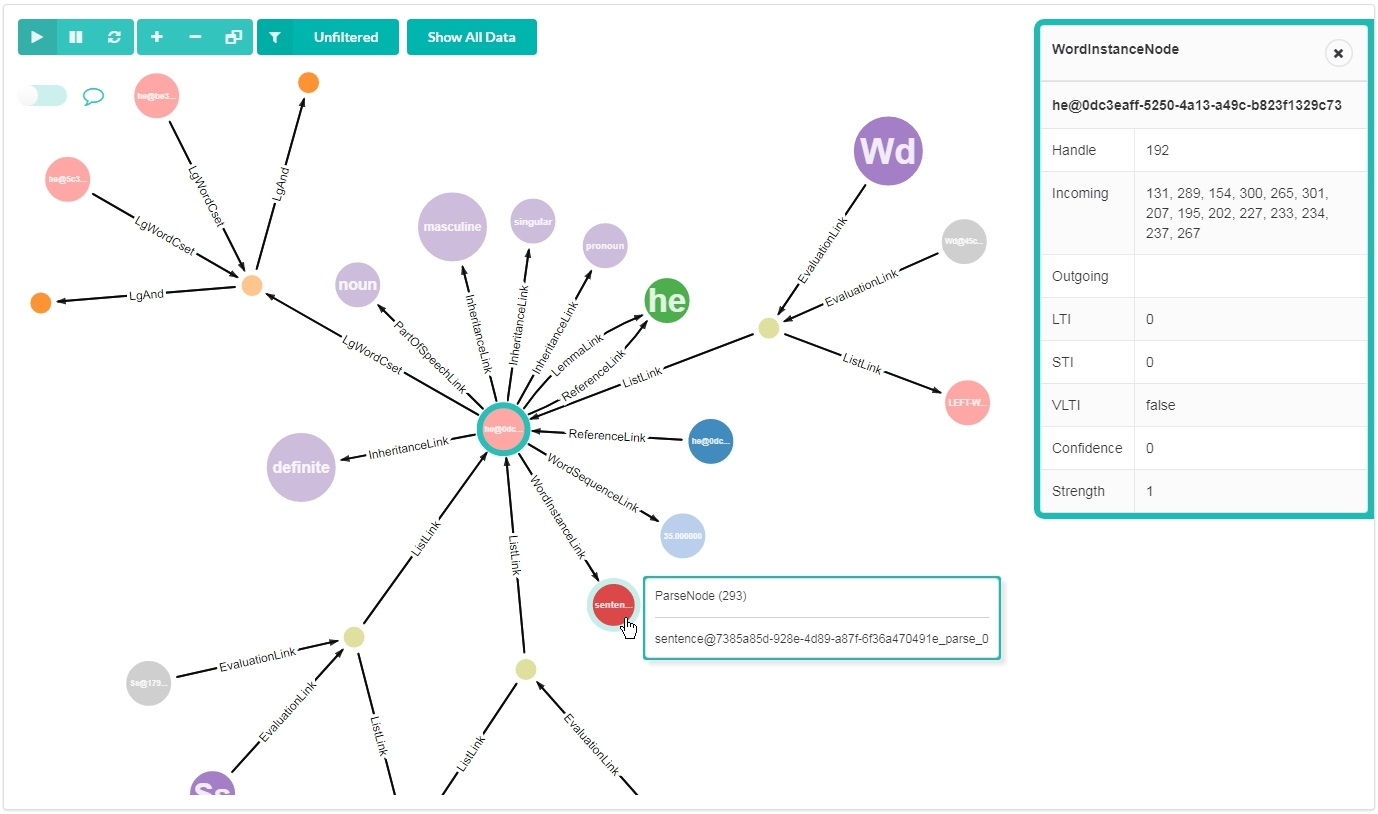
\includegraphics[scale=0.2]{pics/ng2-atomspace-visualizer.jpg}

  \end{columns}

  - - - - - - - - - - - - - - - - - - - - - - - - - - - - - - - - - -
  - - - - - - - - - - - - - - - - - - - - - - - - - - - - - - - - -\\[0.1cm]
  Download docker image: \texttt{\textcolor{black}{sudo docker pull ngeiswei/opencog:agi20}}

\end{frame}

\begin{frame}
  %% I'm gonna give a quit theoretical presentation of what is PLN,
  %% which should help you to understand what's going on during the
  %% tutorial.
  
  \frametitle{PLN}
    - - - - - - - - - - - - - - - - - - - - - - - - - - - - - - - - - -
  - - - - - - - - - - - - - - - - - - - - - - - - - - - - - - - - -\\[0.1cm]
  Download docker image: \texttt{\textcolor{black}{sudo docker pull ngeiswei/opencog:agi20}}

\end{frame}
\end{document}
